\documentclass{article}
\usepackage[utf8]{inputenc}

\documentclass[a4paper]{article}
\usepackage[12pt]{extsizes}
\usepackage{amsmath,amsthm,amssymb}
\usepackage[hidelinks]{hyperref} 
\usepackage[warn]{mathtext}
\usepackage[T1,T2A]{fontenc}
\usepackage[utf8]{inputenc}
\usepackage[english,russian]{babel}
\usepackage{tocloft}
\linespread{1.5}
\usepackage{indentfirst}
\usepackage{setspace}
%\полуторный интервал
\onehalfspacing

\newcommand{\RomanNumeralCaps}[1]
    {\MakeUppercase{\romannumeral #1}}

\usepackage{amssymb}

\usepackage{graphicx, float}
\graphicspath{{pictures/}}
\DeclareGraphicsExtensions{.pdf,.png,.jpg}
\usepackage[left=25mm,right=1cm,
    top=2cm,bottom=20mm,bindingoffset=0cm]{geometry}
\renewcommand{\cftsecleader}{\cftdotfill{\cftdotsep}}

\addto\captionsrussian{\renewcommand{\contentsname}{СОДЕРЖАНИЕ}}
\addto\captionsrussian{\renewcommand{\listfigurename}{СПИСОК ИЛЛЮСТРАЦИЙ}}

\usepackage{fancyhdr}
\usepackage[nottoc]{tocbibind}

\fancypagestyle{plain}{
\fancyhf{}
\renewcommand{\headrulewidth}{0pt}
\fancyhead[R]{\thepage}
}

\usepackage{blindtext}
\pagestyle{myheadings}
\usepackage{hyperref}

\begin{document}
\begin{titlepage}
  \begin{center}
    \large
    Санкт-Петербургский политехнический университет Петра Великого
    
    Институт прикладной математики и механики
    
    \textbf{Высшая школа прикладной математики и вычислительной физики}
    \vfill
    \textsc{\textbf{\Large{КУРСОВАЯ РАБОТ}}}\\[5mm]
    \\ по дисциплине
    \\ <<Математическая статистика>>\\
\end{center}

\vfill

\begin{tabular}{l p{140} l}
Выполнила студентка \\группы 3630102/80401 && Мамаева Анастасия Сергеевна \\
\\
Проверил\\Доцент, к.ф.-м.н.& \hspace{0pt} &   Баженов Александр Николаевич \\\\
\end{tabular}

\hfill \break
\hfill \break
\begin{center} Санкт-Петербург \\2021 \end{center}
\thispagestyle{empty}
\end{titlepage}
\newpage
\newpage
\begin{center}
    \setcounter{page}{2}
    \tableofcontents
\end{center}
\newpage
\begin{center}
    \setcounter{page}{3}
    \listoffigures
\end{center}

\newpage

\section{Постановка задачи}
\noindent Пусть имеется тороидальная камера с магнитными катушками (ТОКАМАК) и детектор-счётчик. В каждый момент времени специальным программным обеспечением получаются сигналы, преобразованные в данные, о текущем местоположении плазмы и количестве выделившихся частиц.

\begin{figure}[H]
		\centering
		\includegraphics[width = 13cm, height = 8cm]{Tokamak.JPG}
		\caption{Схема ТОКАМАКа}
		\label{fig:sP}
	\end{figure}
\noindent В нашей работе необходимо:
\begin{enumerate}
    \item Считать и обработать полученные данные с прибора
    \item Построить графики зависимостей положенения плазмы от времени и количества выделенных нейтронов от времени
    \item Найти функцию корреляции между движением плазмы и количеством вылетающих нейтронов
\end{enumerate}

\section{Теория}
\noindent Часто бывает необходимо определить степень независимости одного процесса от другого или установить сходство одного набора данных с другими. Другими словами, искомой является ыункция корреляции процессов или данных, которую можно определить математически и измерить. Процесс корреляции занимает значимое место в обработке сигналов. Этот математический аппарат нашёл применение в обработке сигналов. Корреляция также является неотъемлемой частью процесса свёртки, который по сути, -- та же корреляция двух последовательностей данных, при вычислении которой одна из последовательностей обращена во времени.

\subsection{Описание корреляции}
\noindent Рассмотрим, как можно сравнить две последовательности данных, состоящие из значений, одновременно выбираемых из двух соответсвующих сигналов. Если два сигнала похоже меняются при переходе от точки к точке, то меру их корреляции можно вычислить, взяв сумму произведений соответсвующих пар точек. Данное предложение становится более аргументированным, если рассмотреть две независимые и случайные последовательности данных. В этом случае сумма произведений стремится к исчезающе малому случайному числу по мере увеличения пар точек. Это объясняется тем, что все числа, положительные и отрицательные, равновероятны, так что пары произведений компенсируются при сложении. В то же время, если сумма конечна, это указывает на наличие корреляции. Отрицательная сумма указывает на отрицательную корреляцию, т.е. увеличение одной переменной связано с уменьшением другой. Таким образом, взаимную корреляцию $r_{12}(n)$ двух последовательностей данных $x_1(n)$ и $x_2(n)$, содержащих по $N$ элементов, можно записать как
$$r_{12}=\sum_{n=0}^{N-1}x_1(n)x_2(n)$$
Однако, такое определение взаимной корреляции даёт результат, который зависит от числа взятых точек. Чтобы это исправить, результат нормируется на число точек. Данную операцию можно рассматривать как усреднение суммы произведений. Получаем следующее улучшенное определение:
$$r_{12}=\frac{1}{N}\sum_{n=0}^{N-1}x_1(n)x_2(n)$$
Впрочем, чтобы данное определение можно было использовать, его также нужно модифицировать. В некоторых случаях корреляция, определенная указанным выше способом, может быть нулевой, хотя две последовательности коррелируют на 100\%. Это может произойти, например, когда два сигнала идут не в фазе (как часто и бывает). Разность фаз может, например, объясняться тем, что $x_1$ -- некий эталонный сигнал, а $x_2$ -- запаздывающий выход схемы. Чтобы преодолеть подобный сдвиг фаз, необходимо сдвинуть (или задержать) один из сигналов относительно другого. Обычно, чтобы выровнять сигналы перед определением корреляции, $x_2$ смещается влево. Это эквивалентно замене $x_2(n)$ на $x_2(n+j)$, где $j$ представляет величину задержки -- число точек выборки, на которое $x_2$ смещается в лево. Альтернативной и эквивалентной процедурой является смещение $x_1$ вправо. В результате получаем такую формулу для взаимной корреляции: 
$$r_{12}(j)=\frac{1}{N} \sum_{n=0}^{N-1}x_1(n)x_2(n+j)=r_{12}(-j)=\frac{1}{N}\sum_{n=0}^{N-1}x_2(n)x_1(n-j)$$
На практике, когда два сигнала коррелируют, их фазовая связь скорее всего неизвестна, так что корреляцию нужно находить для нескольких различных задержек, чтобы установить наибольшее значение корреляции, которое затем считается истинным.
\\
\noindent Разумеется, также можно рассмотреть корреляцию в непрерывной области, и некоторые аналоговые схемы корреляции организованны именно так. В непрерывной области $n \rightarrow t$ и $j \rightarrow \tau$ и 
$$r_{12}(\tau)= \lim_{t \rightarrow \infty} \frac{1}{T} \int_{-\infty}^\infty x_1(t) x_2(t+\tau) dt$$
На практике обрабатываться будут записи конечной длины:
$$r_{12}(\tau)=\frac{1}{T} \int_0^{T} x_1(t) x_2(t+\tau)dt$$

\noindent Есть и другая сложность, связанная с нахождением взаимной корреляции последовательностей данных конечной длины. Если при смещении $x_2$ влево сигналы уже не перекрываются, и данные в конце последовательностей не формируют парные произведения -- возникает так называемый \textit{краевой эффект}. Одно из возможных решений возникшей проблемы заключается в том, чтобы длину одной последовательности сделать в два раза больше длины, необходимой для нахождения корреляции. Для этого можно записать больше данных или, если одна из последовательностей периодична, повторить последовательность. Другое возможное решение -- скорректировать все расчитанные значения.

\subsection{Взаимная корреляция и автокорреляция}
\noindent Определение взаимной корреляции двух периодических последовательностей неравной длины требует аккуратности. Это объясняется тем, что результат корреляции будет повторяться с периодом более короткой последовательности. Этот результат не отражает полной периодичности более длинной последовательности, следовательно, неверен. Продемонстрируем это, найдя взаимную корреляцию $r_{ab}(j)$ последовательностей $a = \{4, 3, 1, 6\}$ и $b = \{5, 2, 3\}$. Последовательность $b$ записывается под $a$ и поэтапно смещается на одну позицию влево, в последнем столбце записываются соответствующие значения взаимной корреляции.
\begin{table}[H]
    \centering
    \begin{tabular}{|c|c|c|}
    \hline 
         последовательность & задержка & $r_{ab}(j)$  \\
         \hline \hline
         4~3~1~6 & & \\
         \hline
         3~5~2~3 & 0 & 47\\ \hline
         5~2~3~5 & 1 & 59\\ \hline
         2~3~5~2 & 2& 34\\ \hline
         3~5~2~3 & 3 & 47\\ \hline
         5~2~3~5 & 4 & 59\\ 
     \hline    
    \end{tabular}
    \label{tab:my_label}
\end{table}
\noindent Результат показывает, что $r_{ab}(j)$ циклично с периодом в три задержки, т.е. период $r_{ab}(j)$ равен периоду более короткой последовательности $b$. Описанная процедура называется \textit{цикличной корреляцией}. Чтобы получить правильное значение, в котором каждое значение $a$ усножается на каждое значение $b$, все элементы $b$ нужно последовательно сместить под каждым значением $a$: 
\begin{figure}[H]
		\centering
		\includegraphics[scale=0.80]{diag.JPG}
		\label{fig:diag}
	\end{figure}
\noindent Видно, что для того, чтобы последовательность $b$ стала повторятться, требуется 6 задержек. Длины последовательностей равны 4 и 3, а число требуемых задержек -- 4 + 3 - 1 = 6. Таким образом, получаем общее правило нахождения линейной взаимной корреляции двух периодических последовательностей длины $N_1$ и $N_2$: дополнить нулями каждую последовательность, чтобы их длины были равны $N_1+N_2-1$ (т.е. добавить $N_2-1$ нулей к последовательности длиной $N_1$ и $N_1-1$ нулей к последовательности длиной $N_2$.) Проиллюстрируем для указанных выше последовательностей:

\begin{table}[H]
    \centering
    \begin{tabular}{|c|c|c|}
    \hline 
         последовательность & задержка & $r_{ab}(j)$  \\
         \hline \hline
         4~3~1~6~0~0 & & \\
         \hline
         5~2~3~0~0~0 & 0 & 29\\ \hline
         2~3~0~0~0~5 & 1 & 17\\ \hline
         3~0~0~0~5~2 & 2 & 12\\ \hline
         0~0~0~5~2~3 & 3 & 30\\ \hline
         0~0~5~2~3~0 & 4 & 17\\ \hline
         0~5~2~3~0~0 & 5 & 35\\ \hline
         5~2~3~0~0~0 & 6 & 29\\
     \hline    
    \end{tabular}
    \label{tab:my_label}
\end{table}
\noindent Следовательно, искомая взаимная корреляция $a$ и $b$ равна
$$r_{ab}(j)=\{29,17,12,30,17,35\}$$

\section{Программная реализация}
\noindent Код программы был написан на языке Python в среде разработки PyCharm. В ходе работы использовались дополнительные библиотеки:
 \begin{enumerate}
        \item seaborn (визуализация)
        \item matplotlib (визуализация)
        \item numpy (вычисление ряда числовых характеристик)
    \end{enumerate}
В приложении находится ссылка на GitHub репозиторий с исходныи кодом.

\section{Ход работы}
\noindent На вход подаётся .txt файл со входными данными, полученными с датчиков ТОКАМАКа. 
\\\\
\noindent Первый этап работы -- обработка информации. Необходимо считать построчно файл, убирая лишние знаки, пробелы и табуляции. Из получившегося массива создать 12 векторов, соответсвующих снятым показаниям.
\\\\
\noindent Второй шаг -- визуализировать обработанные данные. Необходимо построить графики положения плазмы и количества вылетивших нейтронов от момента времени.
\\\\ 
\noindent Третий этап -- построение функций корреляции. Для этого первым делом из векторов, с которыми мы будем работать удалим значения 'NaN', заменив их на 0. Далее напишем функцию сдвига, которая будет в зависимости от значения параметра $\tau$ сдвигать элементы вектора в соответсвующем направлении. Для построения функции корреляции в цикле будем вызывать функцию сдвига shift$(\tau)$, далее перемножать компоненты получившихся векторов между друг другом и суммировать результаты. Полученные результаты будем записывать в массив.
\\\\
\noindent Четвёртый шаг -- нормировка данных. Воспользуемся минмаксной нормализацией, где каждый элемент данных $x$ вычисляется по формуле:
$$x'_i=\frac{x_i - \min(x)}{\max(x)-\min(x)}$$
на выходе получим по оси ординат значения на промежутке [0, 1]
\\\\ 
\noindent Визуализируем полученные данные, сопоставив каждому значению $\tau$ получившееся значение $r_{12}(\tau)$, это и будет график функции взаимной корреляции.

\section{Результаты}
\subsection{Визуализация входных данных}
\begin{figure}[H]
		\centering
		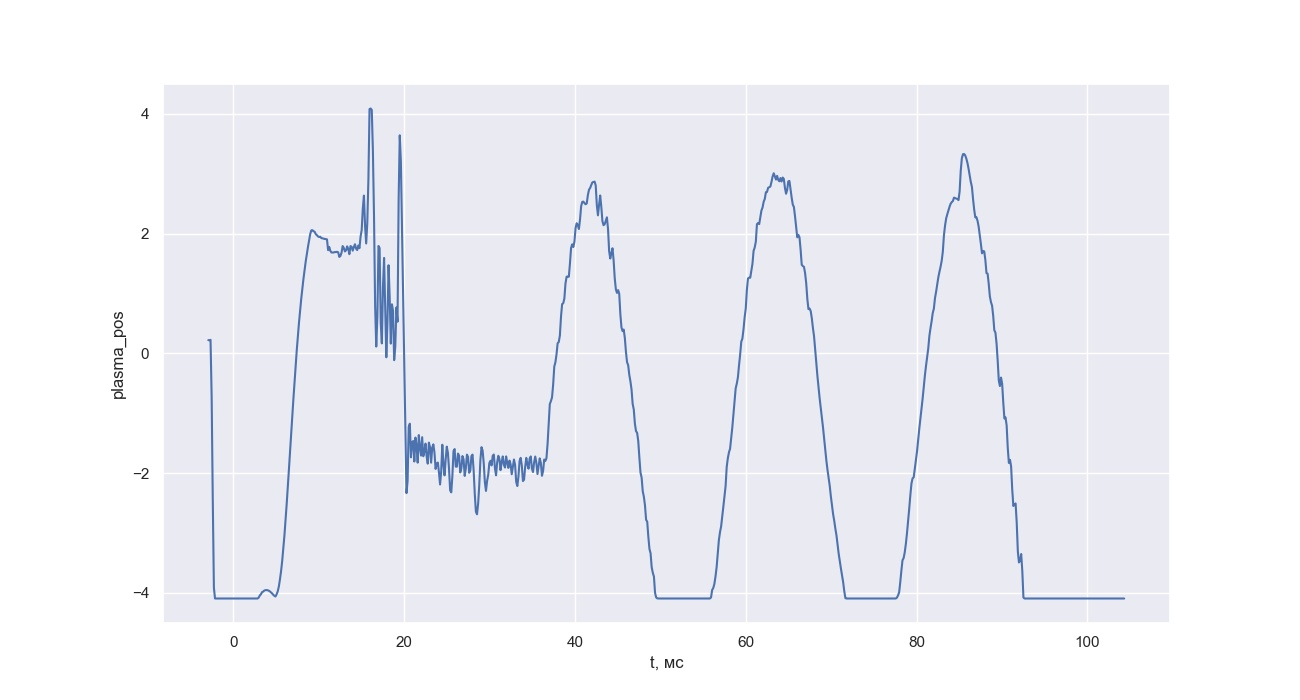
\includegraphics[width = 15cm, height = 9cm]{plasma_pos.jpg}
		\caption{Положение плазмы}
		\label{fig:PP}
	\end{figure}
	
\begin{figure}[H]
		\centering
		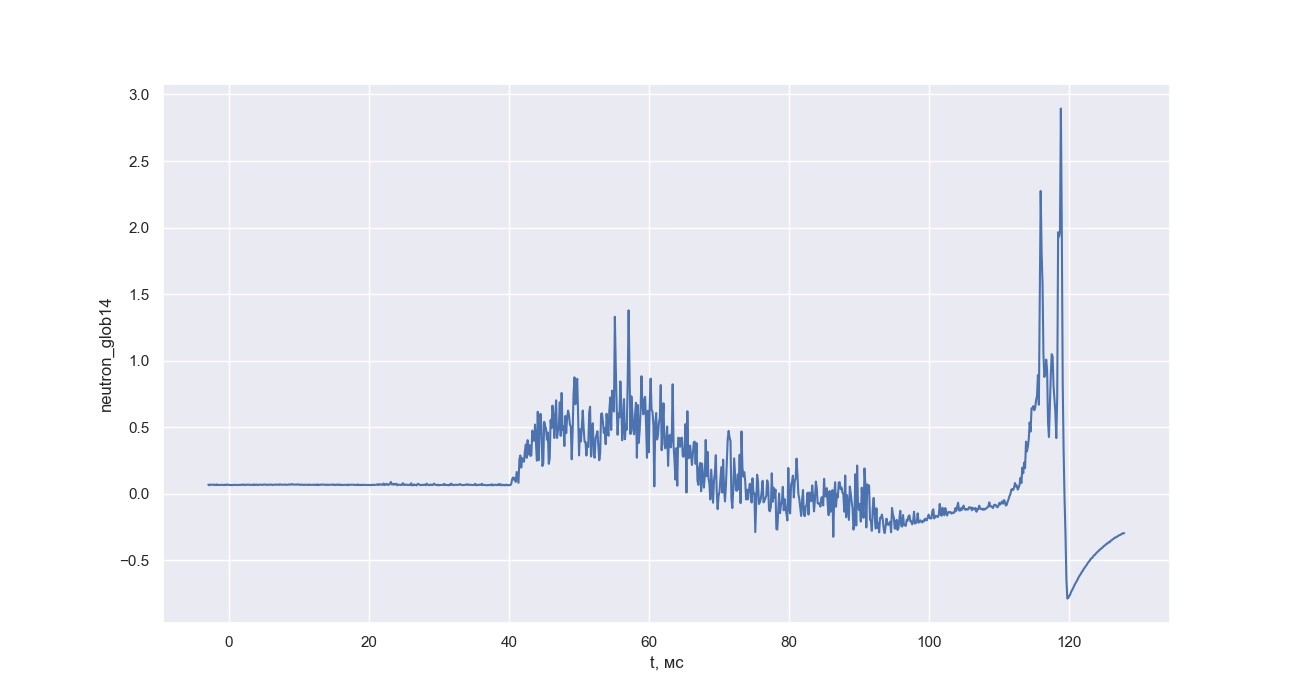
\includegraphics[width = 15cm, height = 9cm]{neutron_glob14, $10^3$.jpg}
		\caption{Количество выделившихся нейтронов\_14}
		\label{fig:NG14}
	\end{figure}
	
\begin{figure}[H]
		\centering
		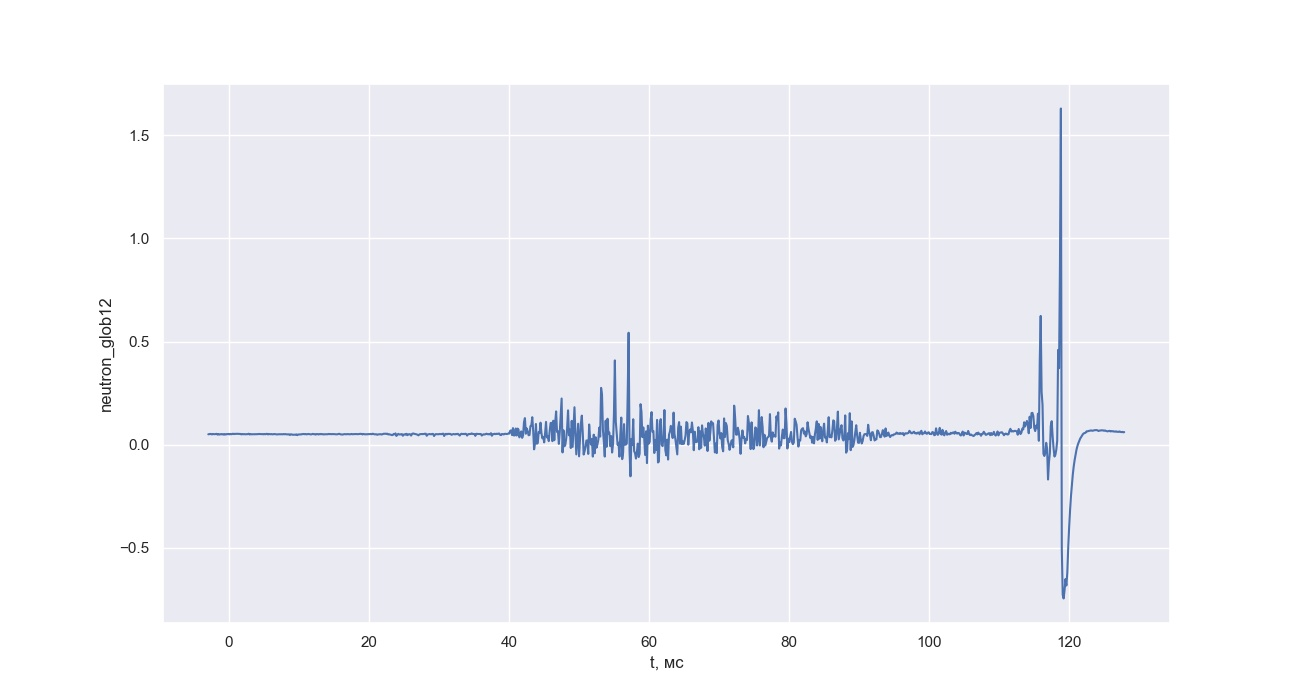
\includegraphics[width = 15cm, height = 9cm]{neutron_glob12, $10^3$.jpg}
		\caption{Количество выделившихся нейтронов\_12}
		\label{fig:NG12}
	\end{figure}

\subsection{Построение функций корреляции}
	
\begin{figure}[H]
		\centering
		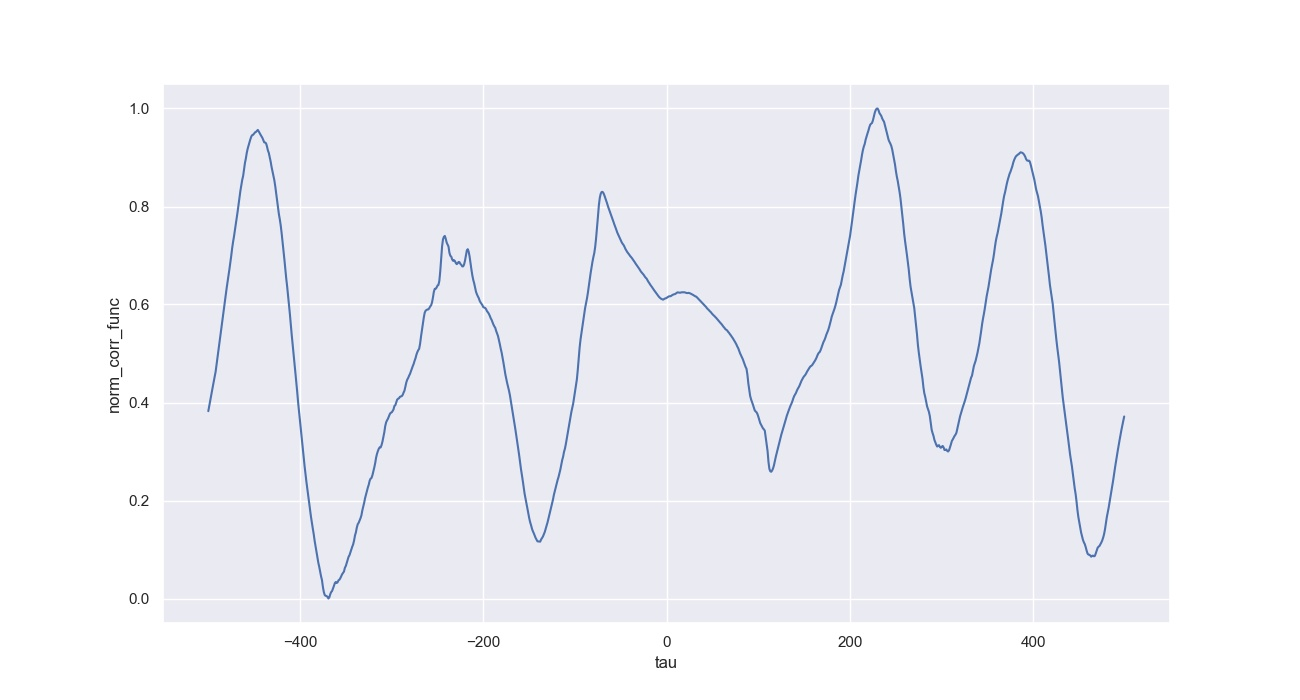
\includegraphics[width = 15cm, height = 9cm]{n_corr_14.jpg}
		\caption{Нормализованная функция взаимной корреляции между плазмой и нейтронами\_14}
		\label{Nc14}
	\end{figure}

\begin{figure}[H]
		\centering
		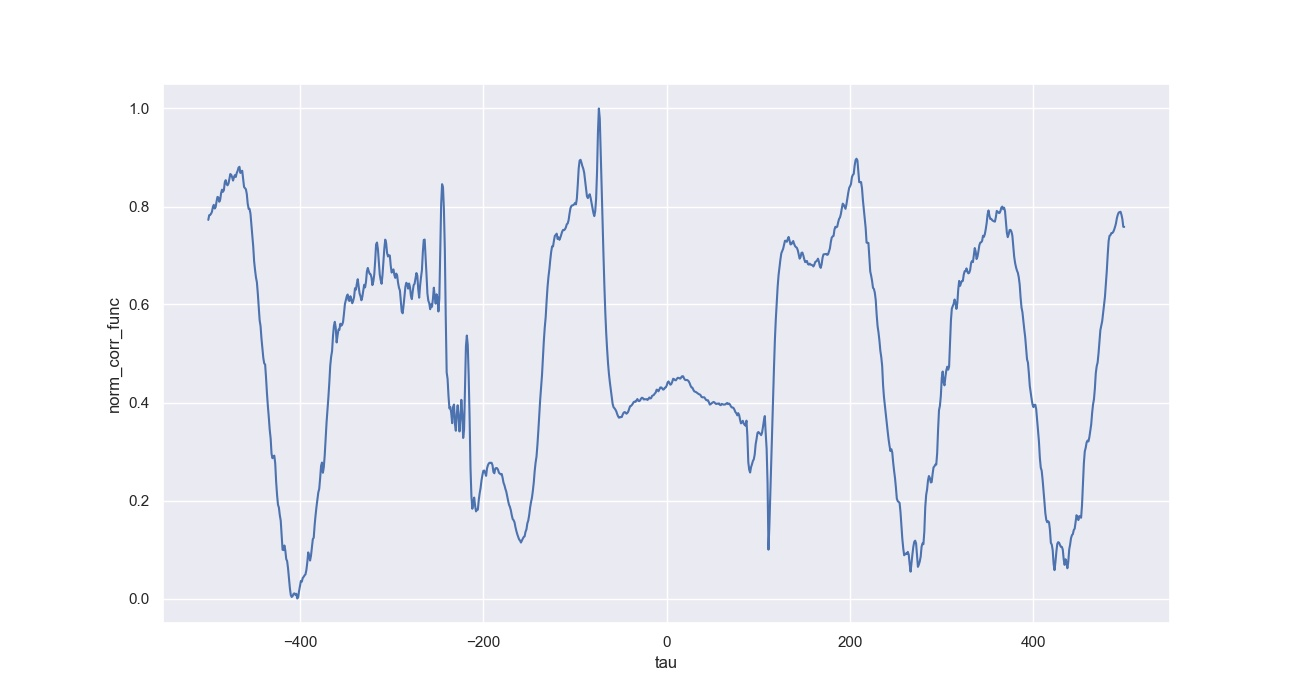
\includegraphics[width = 15cm, height = 9cm]{n_corr_12.jpg}
		\caption{Нормализованная функция взаимной корреляции между плазмой и нейтронами\_12}
		\label{Nc12}
	\end{figure}
	
\section{Анализ}
\begin{enumerate}
    \item При изучении графика \eqref{Nc14} получаем: \\\\
    периодичность $\tau = 210$\\
    основной период колебаний $T=\tau \cdot \Delta t=210\cdot 0.1311мс=27.531мс$\\
    частота колебаний $f=\frac{1}{T}=\frac{1}{27.531}кГц \approx 0.036кГц$\\
    \item Аналогичными выкладками для графика \eqref{Nc12} получаем:\\\\
    периодичность $\tau = -90$\\
    основной период колебаний $T=\tau \cdot \Delta t=90\cdot 0.1311мс=11.799мс$\\
    частота колебаний $f=\frac{1}{T}=\frac{1}{11.799}кГц \approx 0.085кГц$\\
\end{enumerate}
	
\section{Приложение}
\noindent Код программы GitHub URL:\\
\newline https://github.com/Brightest-Sunshine/correlation-analysis-of-plasma/tree/master/scr

\begin{thebibliography}{9}
\bibitem{book1} Вероятностные разделы математики. Учебник для бакалавров технических направлений.//Под ред. Максимова Ю.Д. — Спб.: «Иван Федоров», 2001. — 592 с., илл.
\bibitem{book2} Эконометрика: Учебник/Под ред. И.И. Елисеевой. — М.: Финансы и статистика, 2003. — 344 с.: ил.
\bibitem{book3} Beauchamp K. G. (1973) Signal Processing Using Analog and Digital Techniques. London: Allen and
Unwin
\bibitem{boor4} Электронный ресурс: http://www.williamspublishing.com/PDF/5-8459-0710-1/part.pdf

\end{thebibliography}

\end{document}
